\chapter{Evaluation}
To verify our work on the convergence layer as well as compare it to others and
find potential bottlenecks we evaluated out work under different test cases.
Comparing the data throughput and packetloss for raw IEEE 802.15.4 against DTN
as an additional layer. Distance measurement as well as Round Trip Time
measurement have also been done.

\section{Throughput}
For the real payload data throughput we measured the payload data the receiving
nodes could receive over time. We did the measurement for raw IEEE 802.15.4 and
DTN traffic separately. For both test cases we send packages with the maximum
payload from one node to another as fast as the system allowed. The maximum
payload length for IEEE 802.15.4 packets have been 115 byte and for DTN 40 byte.
That means that for our DTN tests we have a ratio from two third header to one
third payload. As a consequence that results in lower throughput due to less
actual payload can be transmitted in one packet.

During this tests a problem in the lower layers of the system showed up. It is
still unclear if it is a driver or a problem with the ieee802154 stack. The
problem showed up when we tried to send the packets as fast as possible over the
socket interface. After some packets the kernel part got stuck and stopped
transmitting while still accepting data over the socket. The kernel log output
showed a unbalanced IRQ as potential reason for the problem. Time did not allow
to go to the ground of this problem and fix it probably so we went with a delay
in the test application to circumvent this. We added a 100ms delay in the send
routine and the lookup went away. It was the smallest value we could still
reliable send data with. Obviously such a big delay has a negative impact on the
throughput, but without it no measurement would have been possible at all.

Figure \ref{fig:throughput} shows the data we collected with different distances between the
nodes. While the IEEE 802.15.4 throughput gradually goes down the DTN throughput
has some interesting amplitudes and trespasses. We tried to normalize this with
more measurements but every now and then the DTN communication hang up sometimes
for some seconds and then continued. It is yet unknown what part of DTN added
these delays. The new convergence layer would be the first part that needs to be
investigated. Due to the added delay in the testing software the throughput is
not really impressive. The theoretical maximum for IEEE 802.15.4 on the 2.4 GHz
band is about 250 kbps and in our tests we only reached a maximum throughput of
4600 bps.

\begin{figure}
  \begin{center}
    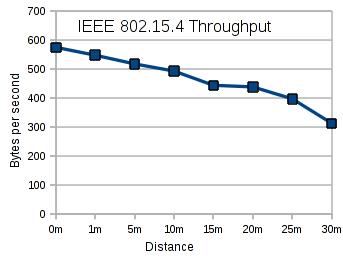
\includegraphics[width=6.5cm]{images/throughput_802154}
    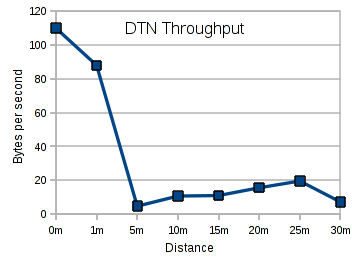
\includegraphics[width=6.5cm]{images/throughput_dtn}
    \caption{Data throughput for IEEE 802.15.4 and DTN}
    \label{fig:throughput}
  \end{center}
\end{figure}

\section{Packetloss}
Throughput alone is of course nothing that tells us much about how reliable a
connection is. Therefor we also measured the packet loss while doing the
throughput measurements. Inside the packet payload a sequence number was encoded
and during a post process the lost packet rate was calculated. No retransmission
was done on the lower layers to avoid even more negative impact on the
throughput and wrong statistics in this test.

Table \ref{tableloss} shows the constant raise of the lost packet rate over the
distance we did our measurements. On a first look it looked suspicious that the
packetloss for DTN was lower then for IEEE 802.15.4 although DTN was used on top
of IEEE 802.15.4. It can be explained though when having in mind that less
packets where send with DTN in the same timeframe. The latency and short hangs
we already discussed did not allow a higher throughput. The slower sending could
explain the better packetloss rate. The single packet had a smaller probability
to get damaged on the air from other packets and thus have a lower packetloss
rate.

\begin{table}
\begin{tabular}{lllllllll}
    & 0m & 1m & 5m & 10m & 15m & 20m & 25m & 30m \\
\hline
802.15.4 & 0\% & 0\% & 10\% & 10\% & 19\% & 20\% & 31\% & 43\% \\
DTN & 0\% & 0\% & 0\% & 15\% & 15\% & 15\% & 20\% & 30\% \\
\end{tabular}
\caption{Packetloss for IEEE 802.15.4 and DTN over distance}
\label{tableloss}
\end{table}

\section{Distance}
The Imote2 has no connector for an external antenna but an on-board antenna
only. To get an understanding what use cases this antenna, and therefor the
whole board, could cover we combined our measurements with a distance
measurement. To decide if a distance is still usable enough we used the
packetloss as quality indicator. All distances which showed a packetloss above
50 percent are rated as unusable. During our measurements such a high packetloss
was shown for all distances higher then 33m.

\section{DTN Round Trip Time}
The last testcase was the round trip time of a DTN bundle. We used the
\emph{dtnping} utility to send out a bundle, receive the answer and calculate
the round trip time. Bundles are send to the \emph{echo} application of the
receiving node. In our case this is directly the DTN daemon. The default payload
size of a ping bundle was to big to our limited payload size on the IEEE
802.15.4 convergence layer. We reduced the payload to 1 byte and used it for all
tests. Table \ref{dtnrtt} shows the results of the measurement in milliseconds. We
had 10 different scenarios for this test case and did five measurements for each.
The first eight are the same we used for our throughput and packetloss test cases.
We added two more scenarios to compare it against our usual test environment as
can be seen in table \ref{dtnrtt2}. The
local scenario did send bundles over the UDP convergence layer on the loopback
interface of our X86 workstation while the UDP scenario did send the bundles
through the UDP convergence layer over an 1 Gbit Ethernet link to another
machine.

The mean round trip time value does not change much from 0m up to 30m. Actually
the values are so near to each other that they can not be rated relevant. That
is of course no real surprise when the maximal distance is as short as 30m. A
delay for the over the air traveling will not be significant on such a distance.

More interesting is the difference between the round trip time on a IEEE
802.15.4 network in contrast to 1 Gbit Ethernet. With a factor of 16 the latency
added by IEEE 802.15.4 is really noticeable. Comparing the value against a
IEEE 802.11 based wirless system could get some insight if this latency is based
on wireless vs. wired or actually on the IEEE 802.15.4 protocol.

\begin{table}
\begin{tabular}{lllllllll}
    & 0m & 1m & 5m & 10m & 15m & 20m & 25m & 30m \\
\hline
Min & 656.14 & 651.11 & 664.25 & 645.27 & 659.29 & 651.40 & 653.66 & 677.29 \\
Mean & 676.17 & 662.38 & 674.85 & 674.85 & 676.46 & 672.03 & 672.47 & 686.60 \\
Max & 693.14 & 678.49 & 684.96 & 685.11 & 695.76 & 684.22 & 687.26 & 693.64 \\
\end{tabular}
\caption{DTN Round Trip Time measurement results over IEEE 802.15.4}
\label{dtnrtt}
\end{table}

\begin{table}
\begin{tabular}{lllllllll}
    & 0m & 1m & 5m & 10m & 15m & 20m & 25m & 30m \\
\hline
Min & 442.41 & 437.44 & 440.15 & 437.58 & 436.88 & 437.76 & 438.57 & 437.82 \\
Mean & 442.53 & 438.29 & 441.36 & 437.65 & 437.68 & 438.54 & 441.46 & 440.94 \\
Max & 442.84 & 438.46 & 443.49 & 441.25 & 442.19 & 441.46 & 441.47 & 441.69 \\
\end{tabular}
\caption{IEEE 802.15.4 Round Trip Time measurement results}
\label{802154rtt}
\end{table}

\begin{table}
\begin{tabular}{lll}
    & Loopback & Ethernet/UDP \\
\hline
Min & 38.31 & 40.90 \\
Mean & 38.87 & 41.26 \\
Max & 39.41 & 41.56 \\
\end{tabular}
\caption{DTN Round Trip Time measurement results over UDP}
\label{dtnrtt2}
\end{table}
